\documentclass[conference]{IEEEtran}
\IEEEoverridecommandlockouts
% The preceding line is only needed to identify funding in the first footnote. If that is unneeded, please comment it out.
\usepackage{cite}
\usepackage{amsmath,amssymb,amsfonts}
\usepackage{algorithmic}
\usepackage{graphicx}
\usepackage{textcomp}
\usepackage{xcolor}
\usepackage{float}
\def\BibTeX{{\rm B\kern-.05em{\sc i\kern-.025em b}\kern-.08em
    T\kern-.1667em\lower.7ex\hbox{E}\kern-.125emX}}
\begin{document}

\title{Analisi esplorativa del tasso di suicidio annuale in diversi paesi su dataset WHO\\
{\footnotesize Tesina di Data Science for Health Systems}
}

\author{\IEEEauthorblockN{Paolo Speziali}
\IEEEauthorblockA{\textit{Dipartimento di Ingegneria} \\
\textit{Università degli Studi di Perugia}\\
Perugia, Italia \\
paolo.speziali@studenti.unipg.it}
}

\maketitle

\begin{abstract}
Questo documento riporta i risultati dell'analisi esplorativa del dataset fornito dalla
World Health Organization relativo al tasso di mortalità per suicidio standardizzato per età.
L'obiettivo di questa analisi è quello di esaminare se, in differenti paesi tra il 2014 e il 2019,
la distribuzione del tasso di suicidi sia significativamente differente o meno,
aprendo la strada a potenziali
ipotesi su fenomeni globali che possono averne influenzato la tendenza.
Tramite l'analisi di tre gruppi distinti è possibile osservare come una
distribuzione senza differenze significative emerga solo in pochi casi.
\end{abstract}

\begin{IEEEkeywords}
suicide, EDA, WHO, GDP
\end{IEEEkeywords}

\section{Introduzione}
Il suicidio è definito come l'atto di terminare intenzionalmente la propria vita\cite{b1}.
Come accade da decenni, il suicidio rimane una delle cause più
frequenti di morte nel mondo occidentale\cite{b2}.
Il Dr. Peeter V\"arnik dell'\emph{Estonian-Swedish Mental Health
and Suicidology Institute}, nel suo paper ``Suicide in the World''\cite{b3}, 
osserva che:
``Il suicidio è un atto individuale ma, una volta che i dati sono aggregati a
livello di paese, le variazioni da un anno all'altro sono piuttosto ridotte e
di solito non ci sono grandi fluttuazioni. Si è tentati di affermare che
il miglior predittore del tasso di suicidi nel breve periodo è il tasso di suicidi del passato.
Tuttavia, nel lungo periodo possono verificarsi e si sono verificati grandi cambiamenti''.
Nello studio che segue andremo ad osservare i cambiamenti nel tasso di suicidio 
a livello mondiale tra il 2000 e il 2019 e verificare se è possibile affermare
che non esistono differenze significative nella distribuzione tassi di suicidio
tra gruppi di paesi differenti.


\section{Dataset}

\subsection{Descrizione del dataset}

Il dataset utilizzato proviene dal portale web della World Health Organization (WHO)
ed ha come titolo ``Age-standardized suicide rates (per 100000 population)''\cite{b4}.
Contiene dati riguardanti i tassi di suicidi in ogni paese dal 2000 al 2019 di soggetti
maschili, femminili e di entrambi i sessi. Tali dati sono standardizzati
prendendo in considerazione la distribuzione dell'età della popolazione del paese,
è stato scelto questo dataset rispetto a ``Crude suicide rates (per 100000 population)''
in quanto la standardizzazione rispetto all'età dà luogo a statistiche più rappresentative
quando l'evento preso in considerazione non è raro\cite{b5}.
I dati sono stati acquisiti attraverso il processo di censimento della popolazione,
registrazioni anagrafiche e l'analisi di certificati medici contenenti informazioni
sulla causa dei decessi.
Il dataset originale si compone di 10980 campioni e 34 feature,
di cui molte con valori totalmente nulli o non importanti ai fini della nostra analisi.

\subsection{Modellazione del dataset}

Prima di iniziare con l'analisi esplorativa il dataset è stato ridotto di
dimensione andando a prendere unicamente le feature d'interesse qui di seguito
riportate:
\begin{itemize}
    \item \textbf{ParentLocation}, rinominato in \textbf{WorldRegion}: 
    indica l'area geografica (World Region o WR) a cui appartiene il paese relativo al dato
    in esame secondo la divisione fatta dalla WHO;
    \item \textbf{SpatialDimValueCode}, rinominato in \textbf{CountryCode}: 
    indica il codice a tre lettere maiuscole associato al paese relativo
    al dato in esame (es. ``Italia'' sarà associato ad ``ITA'');
    \item \textbf{Location}, rinominato in \textbf{Country}: 
    indica il nome del paese  relativo al dato in esame;
    \item \textbf{Period}, rinominato in \textbf{Year}: 
    anno in cui è stato registrato il dato in esame;
    \item \textbf{Dim1}, rinominato in \textbf{Sex}: 
    indica il sesso (Male, Female o Both Sexes)
    relativo al dato in esame;
    \item \textbf{FactValueNumeric}, rinominato in \textbf{Value}: 
    tasso di suicidi registrato per quel sesso in quell'anno e in quel paese.
\end{itemize}
Con le colonne sopracitate selezionate nel dataset non sono presenti
valori nulli o non significativi.
Successivamente il dataset è stato nuovamente modificato per
avere un'unica entry per ogni anno relativo a un paese, suddividendo la feature Sex
in tre feature diverse contenenti ognuna il valore associato nel campo Value.
La struttura finale del dataset, da 3660 campioni e 7 feature, è di seguito riportata:
\begin{itemize}
    \item \textbf{WorldRegion};
    \item \textbf{CountryCode};
    \item \textbf{Country};
    \item \textbf{Year};
    \item \textbf{Male}: Value associato al tasso di suicidio maschile;
    \item \textbf{Female}: Value associato al tasso di suicidio femminile;
    \item \textbf{Both}: Value associato al tasso di suicidio di entrambi i sessi.
\end{itemize}

\section{Analisi esplorativa}

In questa sezione di analisi esplorativa dei dati (EDA) andremo dapprima
ad analizzare tramite strumenti di visualizzazione dei dati il quadro generale
della situazione per poi soffermarci su quattro gruppi di ``soggetti''.

\subsection{Il quadro generale}

Inizialmente è stata studiata la distribuzione dei valori Sex rispetto
al sesso (Male e Female) di appartenenza tramite il boxplot in Fig.~\ref{1sex}.
\begin{figure}[htbp]
    \centerline{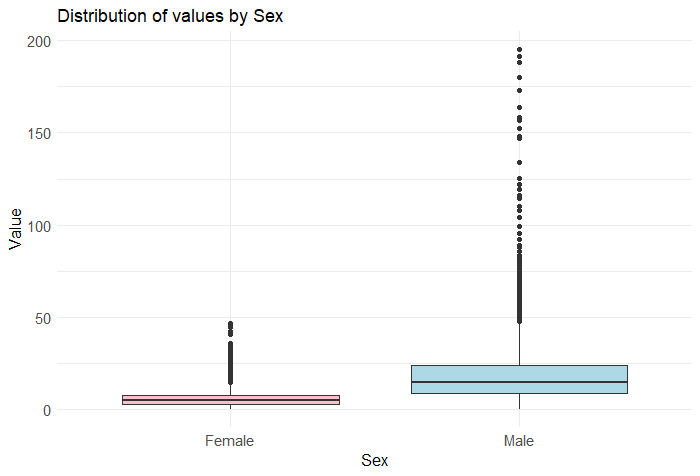
\includegraphics[width=.5\textwidth]{img/1 - Sex2.png}}
    \caption{Boxplot della distribuzione dei valori rispetto al sesso}
    \label{1sex}
\end{figure}
In questo modo è possibile apprezzare come esista una notevole differenza
nella distribuzione tra i sessi: è evidente che i soggetti maschili siano
i più colpiti da questo fenomeno.

\begin{figure}[htbp]
    \centerline{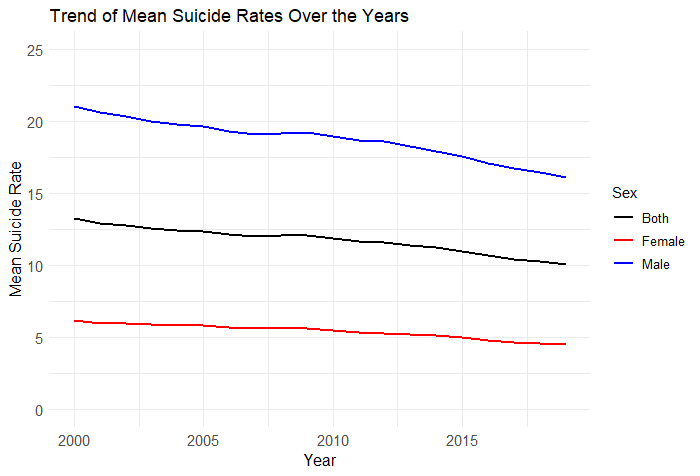
\includegraphics[width=.5\textwidth]{img/2 - Globtrend2.png}}
    \caption{Lineplot del trend dei suicidi medi globali ogni anno}
    \label{2globtrend}
\end{figure}
Ciò è apprezzabile anche andando a vedere il trend globale del
tasso medio dei suicidi ogni anno in Fig.~\ref{2globtrend}: il trend maschile
si trova su valori significativamente più alti rispetto a quello femminile mentre
il trend di Both si pone, prevedibilmente, a cavallo tra i due.

Un'ulteriore osservazione che è possibile fare è
che, nonostante il trend globale sia in declino, non c'è una differenza
particolarmente significativa da anno ad anno. Possiamo apprezzare meglio
ciò osservando la distribuzione dei valori anno per anno tramite il boxplot
in Fig.~\ref{3boxyears}.
\begin{figure}[htbp]
    \centerline{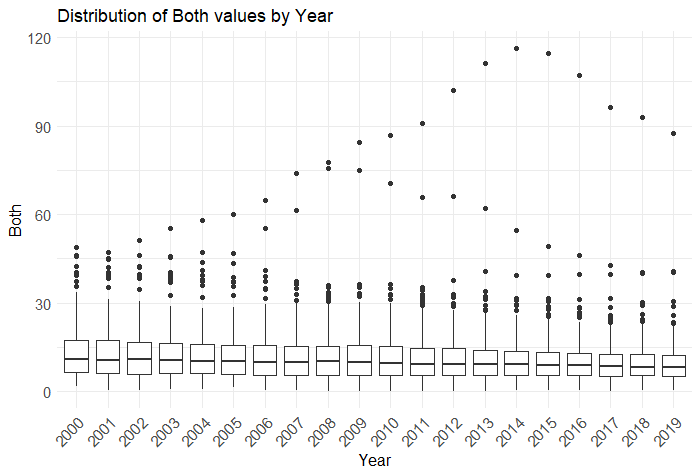
\includegraphics[width=.5\textwidth]{img/3 - Boxyears2.png}}
    \caption{Boxplot della distribuzione dei valori tra gli anni}
    \label{3boxyears}
\end{figure}
La differenza tra un anno e gli adiacenti è poca ma esiste, nel corso del ventennio
in esame infatti la distribuzione cambia notevolmente.
Andiamo infine ad analizzare il trend del tasso dei suicidi medio suddiviso
per regione del mondo secondo la divisione della WHO in Fig.~\ref{4wrtrend}.

\begin{figure}[htbp]
    \centerline{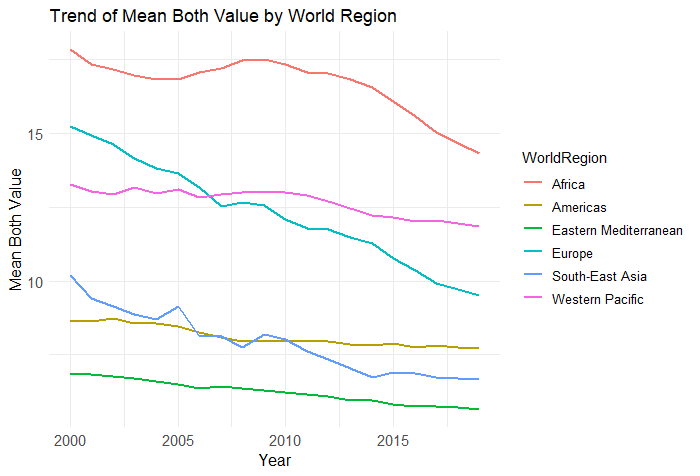
\includegraphics[width=.5\textwidth]{img/4 - WRTrend2.png}}
    \caption{Lineplot del trend dei suicidi medi ogni anno suddiviso per regione globale}
    \label{4wrtrend}
\end{figure}

Possiamo vedere come ci sia in tutte le regioni un trend comune di declino e persino
alcuni trend di crescita e decrescita comuni (ad esempio nel 2008-2009).
A questo punto ci si potrebbe chiedere se alcuni gruppi
di paesi o persino le regioni globali abbiano
distribuzioni di tassi di suicidi senza differenze significative tra loro.

Andiamo ora ad analizzare
un primo gruppo, formato dalle sei regioni globali e dalle loro medie annuali
e poi tre gruppi formati ognuno da sei paesi differenti selezionati con diversi criteri.
Per semplificare l'analisi e ridurre il numero di grafici verranno presi in esame solo
gli anni dal 2014 al 2019.

\subsection{Primo gruppo - Regioni globali (WR)}
Utilizziamo il Box and Whisker Plot (BWPlot) in Fig.~\ref{5firstgroup} per visualizzare il
valor medio di Both in ogni regione del mondo, anno per anno.
\begin{figure}[htbp]
    \centerline{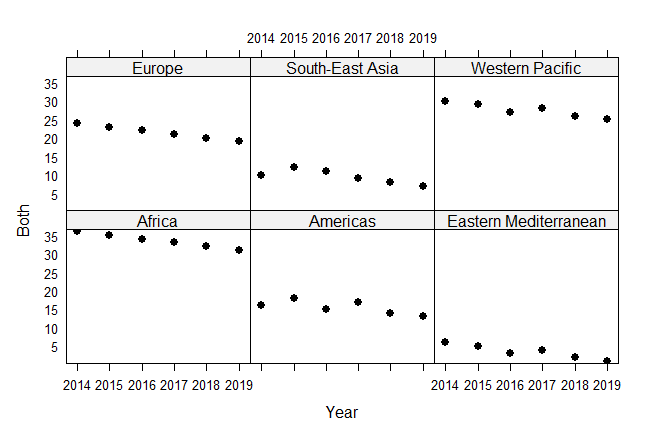
\includegraphics[width=.5\textwidth]{img/5 - Firstgroup.png}}
    \caption{BWPlot della media di Both anno per anno in ogni regione}
    \label{5firstgroup}
\end{figure}
Già dalla figura è possibile vedere che, a parte il declino globale, non viene seguito
un vero e proprio trend comune.
Tramite gli otto QQ-Plot in Fig.~\ref{6firstqq}, uno per anno, si può osservare come sia
molto probabile che le medie dei dati raccolti ogni anno seguano una distribuzione normale.
\begin{figure}[htbp]
    \centerline{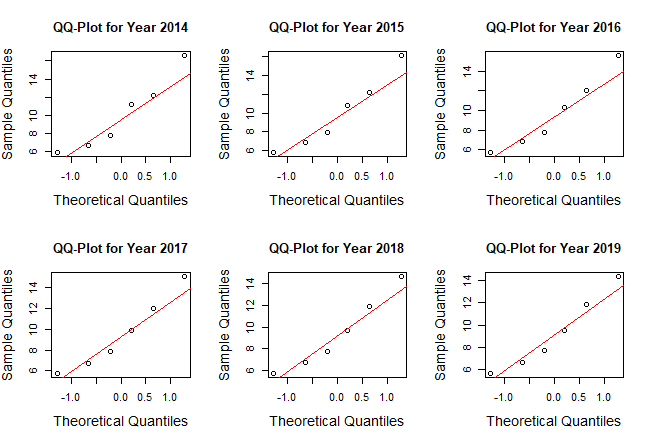
\includegraphics[width=.5\textwidth]{img/6 - Firstqq.png}}
    \caption{QQ-Plot dei valori medi di Both negli anni presi in esame}
    \label{6firstqq}
\end{figure}

\subsection{Secondo gruppo - Paese con PIL più alto per WR}

I paesi individuati come quelli con il PIL maggiore \cite{b6} per la WR
d'appartenenza nel 2019 sono:
\begin{itemize}
    \item \textbf{United States of America} (USA) per Americas;
    \item \textbf{Germany} (DEU) per Europe;
    \item \textbf{China} (CHN) per Western Pacific;
    \item \textbf{Saudi Arabia} (SAU) per Eastern Mediterranean;
    \item \textbf{Nigeria} (NGA) per Africa;
    \item \textbf{India} (IND) per South-East Asia. 
\end{itemize}
Dati questi paesi osserviamo il BWPlot relativo in Fig.~\ref{7secondgroup}.
\begin{figure}[htbp]
    \centerline{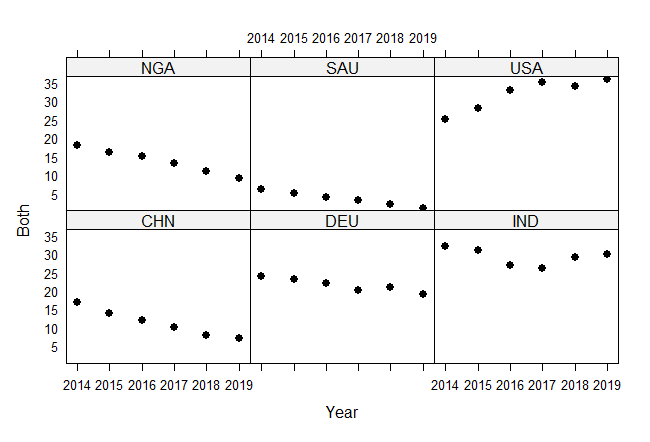
\includegraphics[width=.5\textwidth]{img/7 - Secondgroup.png}}
    \caption{BWPlot di Both anno per anno in ogni paese (2° gruppo)}
    \label{7secondgroup}
\end{figure}
Qua un trend comune appare tra alcuni soggetti mentre tra altri appare di meno,
in seguito verificheremo con un test consono se le distribuzioni differiscono significativamente
tra di loro o meno.
Tramite gli otto QQ-Plot in Fig.~\ref{8secondqq}, uno per anno, si può osservare come, anche qua,
sia molto probabile che i dati raccolti ogni anno seguano una distribuzione normale.
\begin{figure}[htbp]
    \centerline{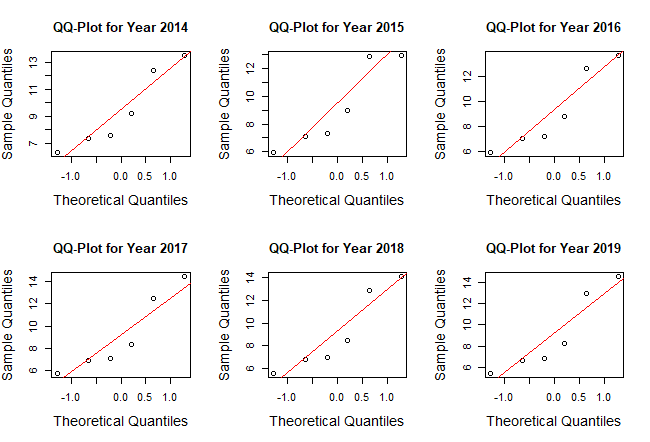
\includegraphics[width=.5\textwidth]{img/8 - Secondqq.png}}
    \caption{QQ-Plot dei valori Both negli anni presi in esame (2° gruppo)}
    \label{8secondqq}
\end{figure}


\subsection{Terzo gruppo - Paesi con tasso di suicidio più alto in assoluto}

I paesi individuati come quelli con il tasso di suicidio più alto
in assoluto sono:
\begin{itemize}
    \item \textbf{Lesotho} (LSO);
    \item \textbf{Guyana} (GUY);
    \item \textbf{Russian Federation} (RUS);
    \item \textbf{Eswatini} (SWZ);
    \item \textbf{Botswana} (BWA);
    \item \textbf{Kiribati} (KIR). 
\end{itemize}
Dati questi paesi osserviamo il BWPlot relativo in Fig.~\ref{9thridgroup}.
\begin{figure}[htbp]
    \centerline{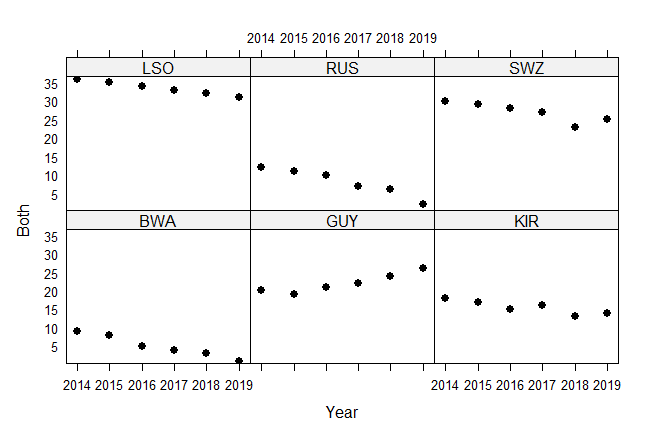
\includegraphics[width=.5\textwidth]{img/9 - Thirdgroup.png}}
    \caption{BWPlot di Both anno per anno in ogni paese (3° gruppo)}
    \label{9thridgroup}
\end{figure}
Qua è difficile individuare un trend comune.
Nei QQ-Plot in Fig.~\ref{10thirdqq} vediamo come i dati non saranno
probabilmente distribuiti normalmente negli anni.
\begin{figure}[htbp]
    \centerline{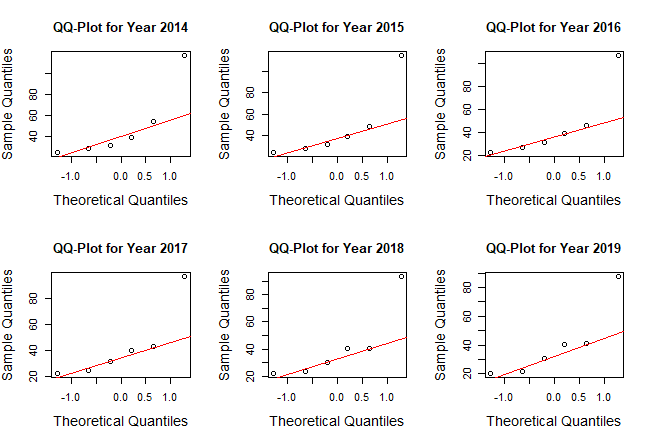
\includegraphics[width=.5\textwidth]{img/10 - Thirdqq.png}}
    \caption{QQ-Plot dei valori Both negli anni presi in esame (3° gruppo)}
    \label{10thirdqq}
\end{figure}

\subsection{Quarto gruppo - Paesi con tasso di suicidio più alto per WR}

I paesi individuati come quelli con il tasso di suicidio più alto per la
WR d'appartenenza sono:
\begin{itemize}
    \item \textbf{Lesotho} (LSO) per Africa;
    \item \textbf{Guyana} (GUY) per Americas;
    \item \textbf{Russian Federation} (RUS) per Europe;
    \item \textbf{Somalia} (SOM) per Eastern Mediterranean;
    \item \textbf{Sri Lanka} (LKA) per South-East Asia;
    \item \textbf{Kiribati} (KIR) per Western Pacific. 
\end{itemize}
Dati questi paesi osserviamo il BWPlot relativo in Fig.~\ref{11fourthgroup}.
\begin{figure}[htbp]
    \centerline{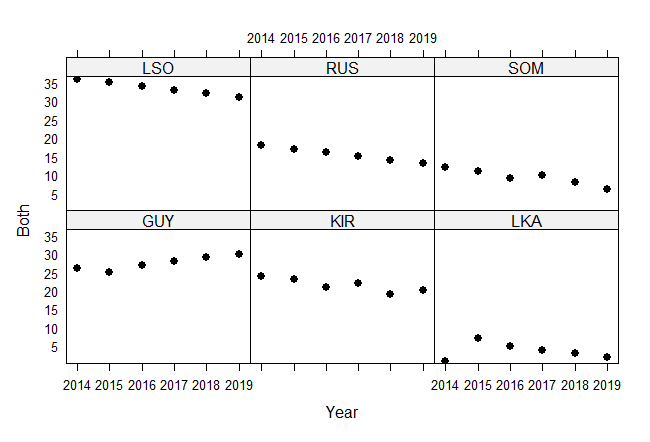
\includegraphics[width=.5\textwidth]{img/11 - Fourthgroup.png}}
    \caption{BWPlot di Both anno per anno in ogni paese (4° gruppo)}
    \label{11fourthgroup}
\end{figure}
Qua un trend comune è già più probabile.
Nei QQ-Plot in Fig.~\ref{12fourthqq} vediamo come i dati non saranno
probabilmente distribuiti normalmente negli anni.
\begin{figure}[htbp]
    \centerline{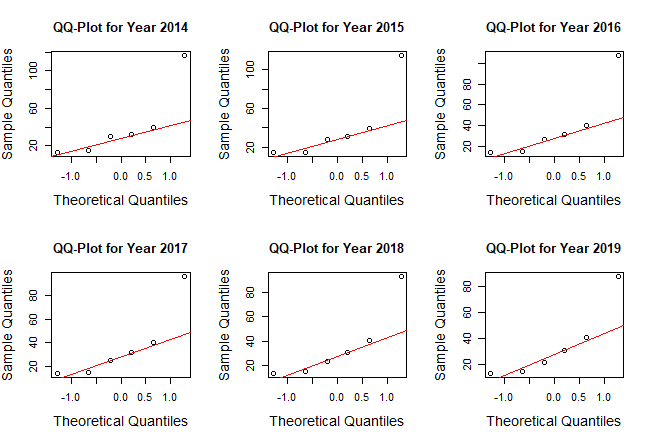
\includegraphics[width=.5\textwidth]{img/12 - Fourthqq.png}}
    \caption{QQ-Plot dei valori Both negli anni presi in esame (4° gruppo)}
    \label{12fourthqq}
\end{figure}

\section{Test statistici}

Vogliamo verificare che, all'interno dei gruppi selezionati,
i dati raccolti provengano da distribuzioni che non differiscono
in maniera significativa tra di loro.
Per fare ciò una buona scelta è l'ANOVA a misure ripetute,
tuttavia è necessario andare a verificare la normalità,
l'omochedasticità e la sfericità delle misure, in caso
anche una sola di queste assunzioni non venga rispettata occorre
ripiegare sul test non parametrico di Friedman.

\subsection{Verifica della normalità}

Le supposizioni sulla normalità dei dati vengono confermate
con il test di Shapiro-Wilk, i cui p-value vengono riportati nella Tab.~\ref{tab1}.
Solo i primi due gruppi presi in esame (gruppo delle medie delle WR e dei paesi con PIL più alto per WR)
infatti rispettano il vincolo della normalità
in quanto hanno tutti i p-value dei test relativi ai loro anni superiori al valore di 0.05.
\begin{table}[htbp]
    \caption{Test di Shapiro-Wilk}
    \begin{center}
    \begin{tabular}{|c|c|c|c|c|c|c|}
    \hline
    \textbf{Gruppo}&\multicolumn{6}{|c|}{\textbf{Anni}} \\
    \cline{2-7} 
     & \textbf{2014} & \textbf{2015} & \textbf{2016} & \textbf{2017} & \textbf{2018} & \textbf{2019}\\
    \hline
    \textbf{Gruppo 1} & 0.531 & 0.672 & 0.690 & 0.705 & 0.708 & 0.719 \\\cline{1-7}
    \textbf{Gruppo 2} & 0.913 & 0.824 & 0.804 & 0.832 & 0.746 & 0.569 \\\cline{1-7}
    \textbf{Gruppo 3} & 0.018 & 0.011 & 0.017 & 0.026 & 0.021 & 0.056 \\\cline{1-7}
    \textbf{Gruppo 4} & 0.015 & 0.011 & 0.018 & 0.037 & 0.046 & 0.071 \\\cline{1-7}
    \hline
    \end{tabular}
    \label{tab1}
    \end{center}
\end{table}

\subsection{Verifica dell'omoschedasticità}

In quanto solo i primi due gruppi hanno dati distribuiti secondo una distribuzione normale
andremo ad utilizzare il test di Bartlett solo su questi due, i risultati,
riportati in Tab.~\ref{tab2}, mostrano come entrambi rispettino l'omoschedasticità.
\begin{table}[htbp]
    \caption{Test di Bartlett}
    \begin{center}
    \begin{tabular}{|c|c|c|}
    \hline
    \textbf{Gruppo} & \textbf{K-squared} & \textbf{p-value} \\
    \hline
    \textbf{Gruppo 1} & 0.27014 & 0.9982 \\\cline{1-3}
    \textbf{Gruppo 2} & 0.39744 & 0.9954 \\\cline{1-3}
    \hline
    \end{tabular}
    \label{tab2}
    \end{center}
\end{table}

Discorso analogo possiamo fare per gli ultimi due gruppi per cui è stato utilizzato il test di
Levene, più robusto rispetto a Bartlett nel caso di allontanamento dalla normalità.
Come si può vedere in Tab.~\ref{tab3}, anche loro sono omoschedastici.
\begin{table}[htbp]
    \caption{Test di Levene}
    \begin{center}
    \begin{tabular}{|c|c|c|}
    \hline
    \textbf{Gruppo} & \textbf{F-value} & \textbf{p-value} \\
    \hline
    \textbf{Gruppo 3} & 0.037 & 0.9992 \\\cline{1-3}
    \textbf{Gruppo 4} & 0.016 & 0.9999 \\\cline{1-3}
    \hline
    \end{tabular}
    \label{tab3}
    \end{center}
\end{table}

\subsection{Verifica della sfericità}

Utilizzando la statistica di Greenhouse-Geisser notiamo come nessuno dei quattro gruppi
soddisfi la sfericità in quanto, i loro valori $\varepsilon$ riportati in Tab.~\ref{tab4},
si allontanano troppo da 1.
\begin{table}[htbp]
    \caption{Statistica di Greenhouse-Geisser}
    \begin{center}
    \begin{tabular}{|c|c|}
    \hline
    \textbf{Gruppo} & $\boldsymbol{\varepsilon}$\\
    \hline
    \textbf{Gruppo 1} & 0.2067 \\\cline{1-2}
    \textbf{Gruppo 2} & 0.2280 \\\cline{1-2}
    \textbf{Gruppo 3} & 0.2122 \\\cline{1-2}
    \textbf{Gruppo 4} & 0.2028 \\\cline{1-2}
    \hline
    \end{tabular}
    \label{tab4}
    \end{center}
\end{table}
Possiamo però pensare di utilizzare comunque ANOVA per i primi due gruppi
che soddisfano sia normalità che omoschedasticità, almeno per vedere
se essa conferma Friedman o meno (in ogni caso, sarà il test di Friedman
quello che considereremo significativo).

\subsection{Test di Friedman}

Per i vari gruppi riportiamo, nella Tab.~\ref{tab5}, i risultati del test di Friedman.
\begin{table}[htbp]
    \caption{Test di Friedman}
    \begin{center}
    \begin{tabular}{|c|c|c|}
    \hline
    \textbf{Gruppo} & $\boldsymbol{\chi}$\textbf{-squared} & \textbf{p-value} \\
    \hline
    \textbf{Gruppo 1} & 26.19 & 8.196$\times 10^{-5}$ \\\cline{1-3}
    \textbf{Gruppo 2} & 10.762 & 0.05631 \\\cline{1-3}
    \textbf{Gruppo 3} & 13.143 & 0.02208 \\\cline{1-3}
    \textbf{Gruppo 4} & 8.2857 & 0.1412 \\\cline{1-3}
    \hline
    \end{tabular}
    \label{tab5}
    \end{center}
\end{table}
Possiamo osservare come solo nel secondo e quarto gruppo 
(ovvero quello dei paesi con PIL più alto per WR e paesi con
suicidio più alto per WR)
il p-value supera il valore di 0.05
e quindi possiamo accettare l'ipotesi nulla, ovvero quella per cui non esistono differenze
statistiche significative all'interno di tali gruppi.
Ciò andrebbe a confermare quel che si poteva leggermente intuire dai BWPlot mostrati per questi
due gruppi.
Nel primo gruppo, ovvero quello composto dalle sei WR e dai rispettivi tassi di suicidio medi per
anno, il p-value è molto più basso rispetto agli altri, indice che
l'evidenza contro l'ipotesi per cui non ci sono differenze significative è forte.
Andando a fare su questo gruppo il
test di Wilcoxon coppia a coppia con la correzione di Benjamini-Hochberg,
i cui p-value sono riportati in Tab.~\ref{tab6} possiamo osservare come
differenze significative si presentino in quasi ogni coppia di anni
messa a confronto.
\begin{table}[htbp]
    \caption{Test di Wilcoxon con correzione di Benjamini-Hochberg}
    \begin{center}
    \begin{tabular}{|c|c|c|c|c|c|}
    \hline
    \textbf{Anni} & \textbf{2014} & \textbf{2015} & \textbf{2016} & \textbf{2017} & \textbf{2018} \\
    \hline
    \textbf{2015} & 0.438 & - & - & - & - \\ \hline
    \textbf{2016} & 0.108 & 0.043 & - & - & - \\ \hline
    \textbf{2017} & 0.078 & 0.043 & 0.438 & - & - \\ \hline
    \textbf{2018} & 0.043 & 0.043 & 0.043 & 0.043 & - \\ \hline
    \textbf{2019} & 0.043 & 0.043 & 0.043 & 0.043 & 0.043 \\ 
    \hline
    \end{tabular}
    \label{tab6}
    \end{center}
\end{table}

\subsection{ANOVA a misure ripetute}

Il primo e il secondo gruppo non rispettano le supposizioni per l'ANOVA a misure ripetute
unicamente perché si allontanano dalla sfericità.
Visti i risultati del test di Friedman, vediamo se l'ANOVA a misure ripetute li conferma
o meno.
In Tab.~\ref{tab7} 
\begin{table}[htbp]
    \caption{ANOVA a misure ripetute}
    \begin{center}
    \begin{tabular}{|c|c|c|}
    \hline
    \textbf{Gruppo} & \textbf{F-value} & \textbf{p-value} \\
    \hline
    \textbf{Gruppo 1} & 4.482 & 0.0878 \\\cline{1-3}
    \textbf{Gruppo 2} & 0.229 & 0.652 \\\cline{1-3}
    \hline
    \end{tabular}
    \label{tab7}
    \end{center}
\end{table}
si osserva come, per entrambi i gruppi, l'ANOVA ci dà un p-value superiore allo 0.05.
Nel secondo gruppo, in cui accettiamo l'ipotesi nulla anche con il test di Friedman,
otteniamo persino uno 0.652.
Nel primo gruppo ci troviamo sopra la soglia con uno 0.0878, con ANOVA quindi
accettiamo l'ipotesi nulla per cui, con Friedman, avevamo una fortissima evidenza contro.
Data però la sfericità non rispettata, i risultati ottenuti con l'ANOVA sono molto
meno significativi.


\section{Conclusioni}

Dall'analisi appena presentata possiamo osservare come, in determinati periodi di tempo
e in determinati gruppi, in questo caso quello dei paesi più ricchi per ogni regione e
quello dei paesi con tasso di suicidio più alto per ogni regione, non esistano differenze
significative nella distribuzione del tasso dei suicidi.
Tuttavia, anche solo il prendere in esame due gruppi con quattro paesi uguali
ma due diversi ci restituisce risultati completamente differenti (ad esempio quanto
visto col terzo e quarto gruppo).
Data la particolarità del fenomeno che può essere attribuito alle motivazioni più disparate,
questa analisi si propone come base per studi futuri, magari andando ad unire questo dataset
con altri dataset che descrivono fattori sociali o geopolitici che potrebbero
essere caratterizzanti per quanto riguarda la distribuzione del tasso dei suicidi.


\begin{thebibliography}{00}
    \bibitem{b1} Shneidman ES. ``The definition of suicide''. New York, NY and London: John Wiley and sons; 1985.
    \bibitem{b2} Gvion Y, Apter A. ``Suicide and suicidal behavior''. Public Health Reviews. 2012;34: epub ahead of print.
    \bibitem{b3} Värnik, P. ``Suicide in the world''. Int. J. Environ. Res. Public Health 2012, 9, 760-771. https://doi.org/10.3390/ijerph9030760 
    \bibitem{b4} World Health Organization. (2023). ``Suicide rates''. Recuperato da https://www.who.int/data/gho/data/themes/mental-health/suicide-rates
    \bibitem{b5} Statistics Canada. (2023). ``Age-standardized rates''. Recuperato da https://www.statcan.gc.ca/en/dai/btd/asr
    \bibitem{b6} countryeconomy.com. (2023). ``GDP - Gross Domestic Product 2019''. Recuperato da https://countryeconomy.com/gdp?year=2019
\end{thebibliography}

\end{document}
